%Wf4ever Main Document File
\documentclass[a4paper, twoside, 11pt]{article}

\usepackage[scaled=0.92]{helvet}
\usepackage{fancyhdr}
\usepackage{courier}
\usepackage{caption}
\usepackage{subcaption}
%\usepackage{subfigure}
\normalfont % in case the EC fonts aren't available
\usepackage[T1]{fontenc}
\parskip=2pt\parindent 0pt


\usepackage{url}
\usepackage{listings}
\usepackage{inconsolata}
\usepackage{hyperref}
\usepackage{wf4ever}
\usepackage{xspace}
\usepackage{amsfonts}
\usepackage{amssymb}
\usepackage{amsmath}
\usepackage{verbatim}

\usepackage{color}
%figure with pdf latex
\usepackage[pdftex]{graphicx}
\usepackage{epstopdf}
\DeclareGraphicsExtensions{.jpg,.pdf,.png}

% Macros

% Identifying documents

\id{2.2v2}
\idyear{2013} %To adjust year for "Document Identifier"
\title{D\delid\ Design, implementation and deployment of workflow
  lifecycle management components - Phase II}
\coordinator{Khalid Belhajjame} %Del Coordinator
\institution{University of Manchester} %Del Coordinating Inst.
\authors{Daniel Garijo, Graham Klyne} %Other authors
\abstract{This deliverable describes the second phase of delivery of
  workflow lifecycle management components. It includes a description
  of the Research Object Model, which facilitates interoperation
  between components; the RO Manager command line tool; the Research Object Digital Library; the RO-enabled myExperiment; and a definition of models for
workflow abstraction and indexation.}
\version{0.1} %Please fill out version
\datesubmitted{June 30, 2013} %Submission date
\datedue{June 30, 2013} %Date due
\state{Draft} %State
\distribution{Public} %Distribution (Public, Restricted, Confidential)

\copyrighty{2013}



\begin{document}
\maketitle


\section*{Work package participants} The following partners have taken an active part in the work leading to the elaboration of this document, even if they might not have directly contributed to the writing of this document or its parts: %Enter Work Package Participants:
\begin{itemize}
\item iSOCO
\item OXF
\item PSNC
\item UNIMAN
\item UPM
\end{itemize}

\section*{Change Log}
%Fill in table
\begin{centering}

\begin{tabular}{|c|c|p{4.92cm}|p{6.5cm}|}

\hline \textbf{Version} & \textbf{Date} & \textbf{Amended by} & \textbf{Changes} \\ \hline
0.1 & 01-06-2013 & Khalid Belhajjame & Initial outline \\ \hline
0.2 & 09-06-2013 & Khalid Belhajjame & Initial draft of Section 2 on the RO model \\ \hline
0.3 & 12-06-2013 & Graham Klyne & Added the RO manager section \\ \hline
0.4 & 14-06-2013 & Daniel Garijo & Added the workflow abstraction section \\ \hline
0.5 & 14-06-2013 & Khalid Belhajjame & Added the introduction and a first draft of the myExperiment section \\ \hline
0.6 & 14-06-2013 & Khalid Belhajjame & Revised all sections and added the summary section \\ \hline
0.7 & 21-06-2013 & Khalid Belhajjame & Addressed QA comments received from Oscar Corcho on all sections, except Sections 4 and 7 \\ \hline
0.8 & 21-06-2013 & Raul Palma & Research Object Digital Library section \\ \hline
0.8.1 & 21-06-2013 & Piotr Ho\l{}ubowicz & Research Object Digital Library UML diagrams and alignment\\ \hline
0.8.2 & 24-06-2013 & Raul Palma & Research Object Digital Library section references and fixes\\ \hline
%&&&\\ \hline
%&&&\\ \hline

\end{tabular}

\end{centering}
\clearpage
\section*{Executive Summary}
%Please enter Executive Summary
This deliverable describes the second phase of delivery of workflow
lifecycle management components. These components are focused around
the Wf4Ever Research Object Model (RO Model), which provides
descriptions of workflow-centric ROs -- aggregations of content. This
model is used to structure and describe ROs which are then stored and
manipulated by the components of the Wf4Ever Toolkit.

The RO Model provides a framework for describing aggregations of
content along with annotations of the aggregated resources, a
vocabulary for describing workflows, and a vocabulary for describing
provenance. The model did not undergo any major changes in the in the last year, which is a good sign as it suggests that the model is mature enough and captures user requirements adequately. 
We provide here a description of the RO model.
We also present the components developed for creating and managing Research Objects: the
RO Manager -- the
Research Object Digital Library. These components and services are also discussed in D1.2v3
(Wf4Ever Sandbox -- Phase II), D1.3v2 (Wf4Ever Architecture -- Phase
II) and D1.4v2 (Reference Wf4Ever Implementation -- Phase II). 

One of the main developments in the last year consist in incorporating research objects within the myExperiment environment to allow scientists who already use myExperiment to create, share and reuse research objects. We discuss the efforts that went into this task, and show how myExperiment is using Research Object Digital Library as a back-end for storing and archiving Research Objects.

We  present advanced management functions that we developed for abstracting and indexing workflows, with the aim of supporting the discovery and reuse of workflows. We present an ontology that we developed for abstracting workflows in terms of motifs that characterize data manipulation and transformation patterns, which we term motifs. We also report on a solution that we developed for indexing workflows based on the services (processes) that they use.

This deliverable should be read in tandem with D1.3v2 (Wf4Ever
Architecture -- Phase II), D1.4v2 (Reference Wf4Ever Implementation --
Phase II), D1.2v3 (Wf4Ever Sandbox -- Phase III), D3.2v2 (Design,
implementation and deployment of Workflow Evolution, Sharing and
Collaboration components -- Phase II) and D4.2v2 (Design,
implementation and deployment of Workflow Integrity and Authenticity
Maintenance components -- Phase II) in order to provide a complete
picture of the state of the Wf4Ever Phase II components.

\clearpage

\tableofcontents
\clearpage
%\listoftables %Add comment to suppress list of tables
\listoffigures %Add comment to suppress list of figures

\section*{List of Ontologies}
\begin{enumerate}
\item
\texttt{RO} ontology: \url{http://purl.org/wf4ever/ro#}
\item
\texttt{Wfdesc} ontology: \url{http://purl.org/wf4ever/wfdesc#}
\item
\texttt{Wfprov} ontology: \url{http://purl.org/wf4ever/wfprov#}
\item
\texttt{ROEvo} ontology: \url{http://purl.org/wf4ever/roevo#}
\end{enumerate}


\clearpage
\sloppy

%Your work starts here

\section{Introduction}

This deliverable describes aspects of Phase I of the design,
implementation and deployment of the Wf4Ever components that will
support workflow lifecycle management. The document should be read in
tandem with other Month 20 deliverables, in particular
D3.2v1~\cite{D3.2v1} and D4.2v1~\cite{D4.2v1} which adress
complementary aspects of the overall wf4ver architecture and
components.

According to the Description of Work, \emph{This prototype will
  include the following functionalities: an initial Research Object
  model, implemented by means of an ontology network, and basic
  management functions (storage and access), validation
  functionalities based on RO provenance, and definition of semantic
  overlays and workflow provenance matching techniques for
  abstraction.}. 

These requirements are addressed in the following way:

Sections~\ref{sec:model}, \ref{sec:primer} and \ref{sec:examples}
discuss the Research Object Model defined within Wf4Ever along with a
Primer document providing an introduction to that model and a
collection of example Research Objects. 

Sections~\ref{sec:rosrs} and \ref{sec:manager} describe the initial
Research Object Storage and Retrieval Service and Command Line
Manager. Both of these tools use the Research Object Model to
structure the objects that they produce and consume. The RO Model is
thus the ``glue'' that joins together the components and enables
interoperation. 

Section~\ref{sec:abstraction} discusses an initial model for workflow
abstraction, while Section~\ref{sec:decay} presents a characterisation
of workflow decay. 

Note that this document represents the results from Phase I of the
project -- as a result, some areas are not yet complete and we expect
updates, changes and extensions to be reported in Phase II of the
project, due for completion in M32. For example, we expect that RO models reported
here will be subject to change following further usage and experience,
both within and outside the project.

\section{The Research Object Model}
\label{sec:romodel}

The design of the Research object model was informed by a systematic analysis of requirements expressed by scientists from the life sciences and astronomy fields. The results of such analysis are summarised in Figure \ref{fig:wm_abstract}, which distinguishes between core and extended requirements. There are three core requirements that have been identified, namely a mechanism for uniquely identifying Research Objects, a means for aggregating resources within a Research Object, and the ability to annotate the Research Object, its constituent resources and their relationships. Based on the core requirements, the extended requirements highlight the need for specifying workflows (experiments), provenance traces of their executions, the evolution of a Research object over time, as well as mechanisms for citing Research Objects, expressing their dependencies, etc.


\begin{figure}[ht]
  \centering
  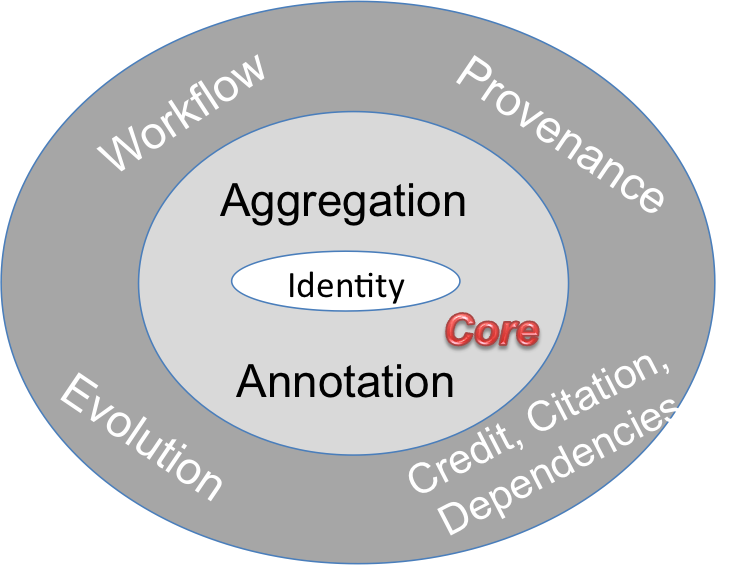
\includegraphics[width=0.4\textwidth]{Figures/wm_abstract.png}
  \caption{Research Objects: Abstract model.}
  \label{fig:wm_abstract}
\end{figure}

We have realized the Research Object abstract model illustrated in Figure \ref{fig:wm_abstract} in the form of a family of ontologies that are illustrated in Figure \ref{fig:wm_concrete}, which we will present in the rest of this section.  It is worth noting that some of the vocabularies, e.g., ORE\footnote{\url{www.openarchives.org/ore}} and OA ~\cite{COG11}, are existing vocabularies that we built on to specify our ontologies.

 \begin{figure}[ht]
  \centering
  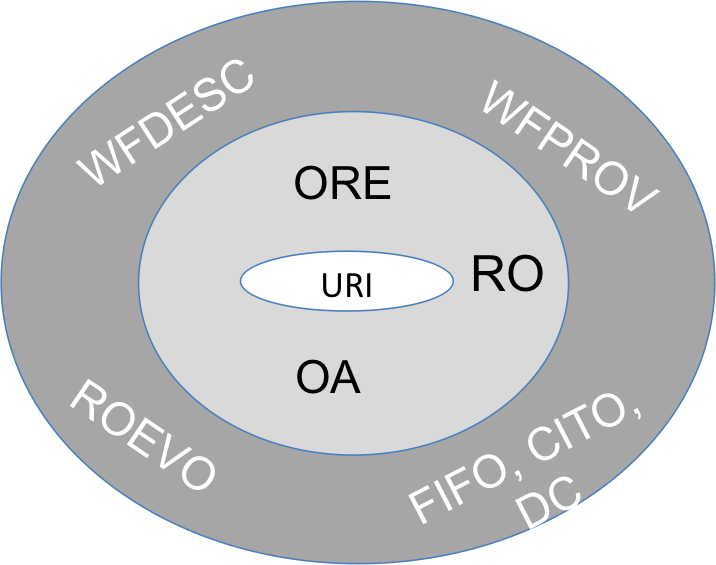
\includegraphics[width=0.4\textwidth]{Figures/wm_concrete.png}
  \caption{Research Objects: Concrete model.}
  \label{fig:wm_concrete}
\end{figure}

\subsection{RO core ontology} 
The Core RO Ontology provides the minimum terms that are essential to the specification of research objects. Specifically, it caters for two essential requirements by providing a container structure that can be used by the scientists to bundle the resources and material relevant for their investigation, and by enabling annotations of such a container, its resources, as well as the relationships between resources thereby making the research object interpretable and reusable. 

To cater for the specification of aggregation structures, we built the Research Object Core Ontology upon the popular ORE vocabulary. ORE defines standards for the description and exchange of aggregations of Web resources. 
Figure \ref{fig:ro_ontology} illustrates the main terms that constitute the Research Object Core Ontology, which we describe in what follows.


\begin{figure}[ht]
  \centering
  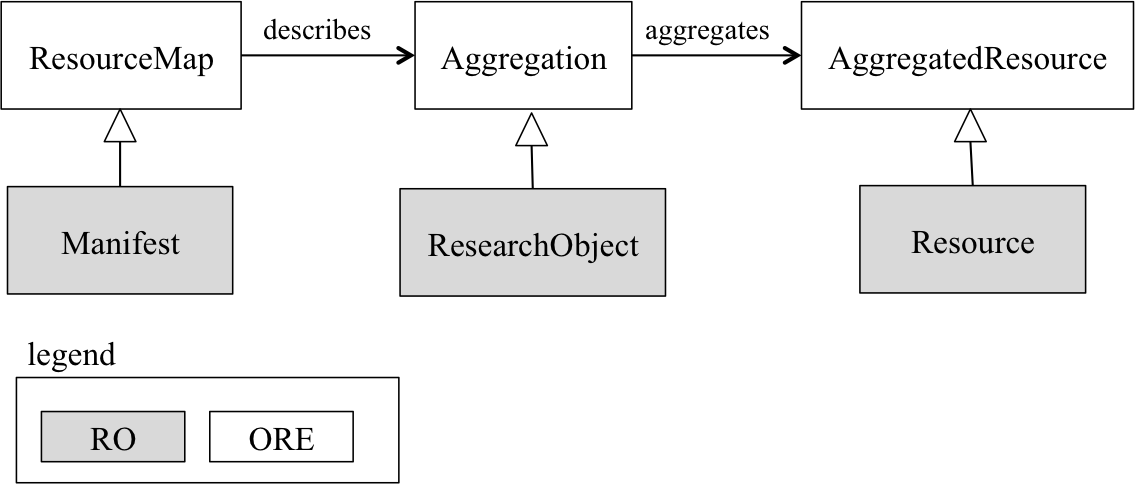
\includegraphics[width=0.6\textwidth]{Figures/ro_ontology_1.png}
  \caption{RO as an ORE aggregation.}
  \label{fig:ro_ontology}
\end{figure}

\begin{itemize}
\item
\texttt{ro:ResearchObject}\footnote{The namespace of the Research Object Core Ontology \texttt{ro} is \url{http://purl.org/net/wf4ever/ro\#}}, represents an aggregation of resources. It is a sub-class of \texttt{ore:Aggregation} and acts as an entry point to the research object.
\item
\texttt{ro:Resource}, represents a resource that can be aggregated within a research object and is a sub-class of \texttt{ore:AggregatedResource}. A resource can be a Dataset, Paper, Software or Annotation. Typically, a \texttt{ro:ResearchObject} aggregates multiple \texttt{ro:Resource}, and this relationship is specified using the property \texttt{ore:aggregates}.
\item
\texttt{ro:Manifest}, a sub-class of \texttt{ore:ResourceMap}, represents a resource that is used to describe a \texttt{ro:ResearchObject}. It plays a similar role to the manifest in a JAR or a ZIP file, and is primarily used to list the resources that are aggregated within the research object.
\end{itemize}

The second core requirement that, the Research Object Core Ontology caters for, is the descriptions of the research object and its elements. We chose the Annotation Ontology (AO) release 2.0b2~\cite{COG11}.To annotate research objects, we make use of the following three Annotation Ontology terms \texttt{ao:Annotation}\footnote{The namespace of \texttt{ao} is \url{http://purl.org/ao/}}, which represents the annotation itself; \texttt{ao:Target}, which is used to specify the \texttt{ro:Resource}(s) or \texttt{ro:ResearchObject}(s) subject to annotation; and \texttt{ao:Body}, which comprises a description of the target.
In the case of research objects, we use annotations as a mean for decorating a resource (or a set of resources) with metadata information. The body is specified in the form of a set of RDF statements, which can be used to, e.g., specify  the date of creation of the target or its relationship with other resources or research objects. Also, annotations can be provided for human consumption (e.g. a description of a hypothesis that is tested by a workflow-based experiment), or for machine consumption (e.g. a structured description of the provenance of results generated by a workflow run). Both kinds of annotations are accommodated using Annotation Ontology structures.

\subsection{RO Extension Ontologies}
We present in this section two  extensions to the core Research Object ontology. The first specializes the kinds of resources that the research object can aggregate. In particular, we present extensions to specify  method and experiments and the traces of their executions. The second kind of extension shows how specific metadata information, specifying the evolution of the research object over time, can be specified by specializing the Research Object core ontology.

\paragraph{Specifying Workflows}
To describe workflow research objects the workflow description vocabulary \textit{wfdesc}\footnote{The name space of \textit{wfdesc} is \url{http://purl.org/wf4ever/wfdesc\#}.} defines several specific resources that are involved in a workflow specification. The choice of these resources was performed by examining the commonalities between major data driven workflows, namely Taverna\footnote{http://www.taverna.org.uk}, Wings\footnote{http://http://wings-workflows.org} and Galaxy\footnote{http://galaxyproject.org}, to cite a few.

\begin{figure}[ht]
  \centering
  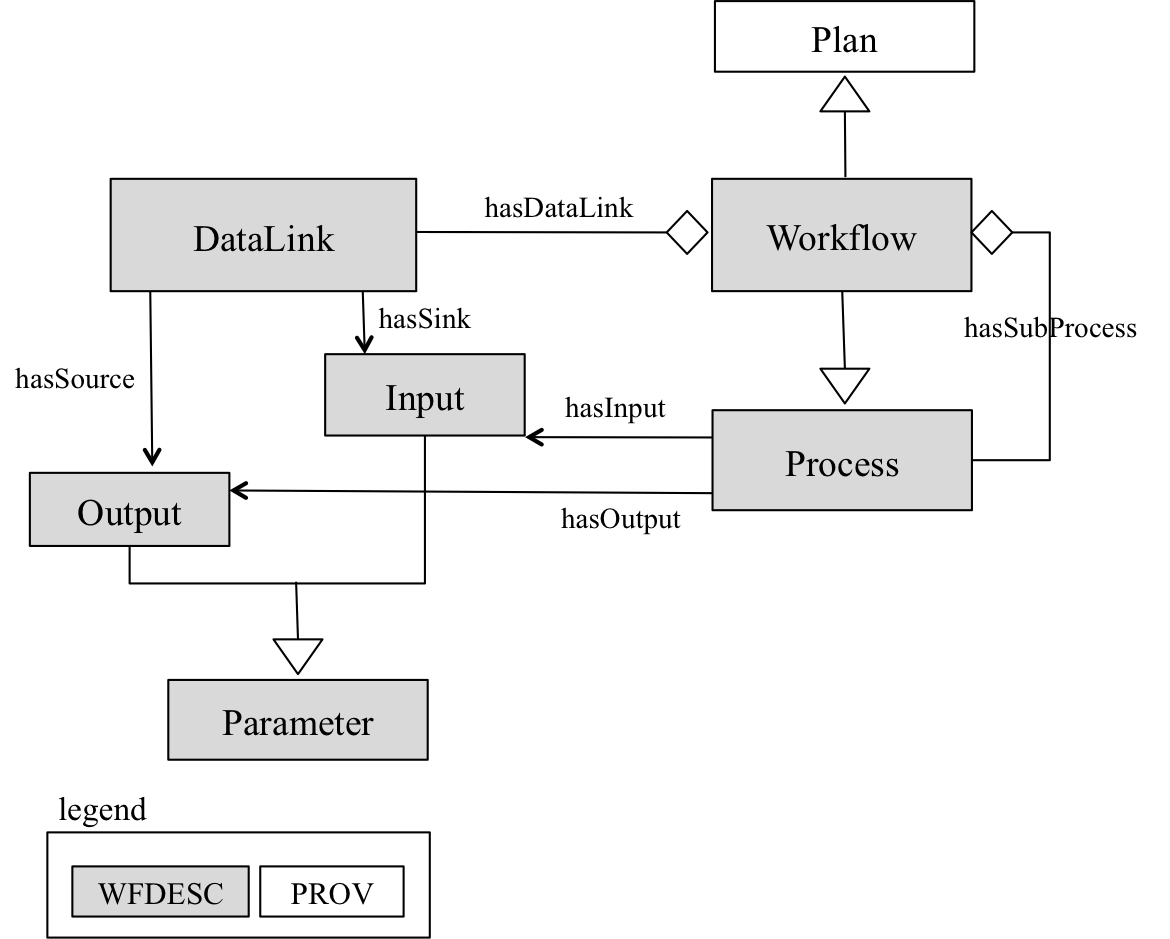
\includegraphics[width=0.6\textwidth]{Figures/wfdesc.png}
  \caption{The \textit{wfdesc} ontology.}
  \label{fig:wfdesc}
\end{figure}

Figure \ref{fig:wfdesc} illustrates the terms that compose the \textit{wfdesc} ontology. Using such ontology, a workflow is described using the following three main terms:
\begin{itemize}
\item
\texttt{wfdesc:Workflow} refers to a network in which the nodes are processes and the edges represent data links. It is defined as a subclass of the \textit{Plan} concept from the PROV-O ontology, which represents a set of actions or steps intended by one or more agents to achieve some goals \cite{w3c-prov-o}. 
\item
\texttt{wfdesc:Process} is used to describe a class of actions that when enacted give rise to process runs. Processes specify the software component (e.g., web service) responsible for undertaking those actions.
\item
\texttt{wfdesc:DataLink} is used to encode the data dependencies between the processes that constitute a workflow. Specifically, a data link connects the output of a given process to the input of another process, specifying that the artifacts produced by the former are used to feed the latter.
\end{itemize}


\paragraph{Describing Experimental Provenance using the \textit{wfprov} Vocabulary}
The \textit{wfprov} ontology is used to describe the provenance traces obtained by enacting  workflows. It is defined as an extension to the ongoing W3C PROV standard ontology - PROV-O\footnote{Note that the \textit{wfprov} is reported in the W3C PROV Working Group implementation report.}.

\begin{figure}[ht]
  \centering
  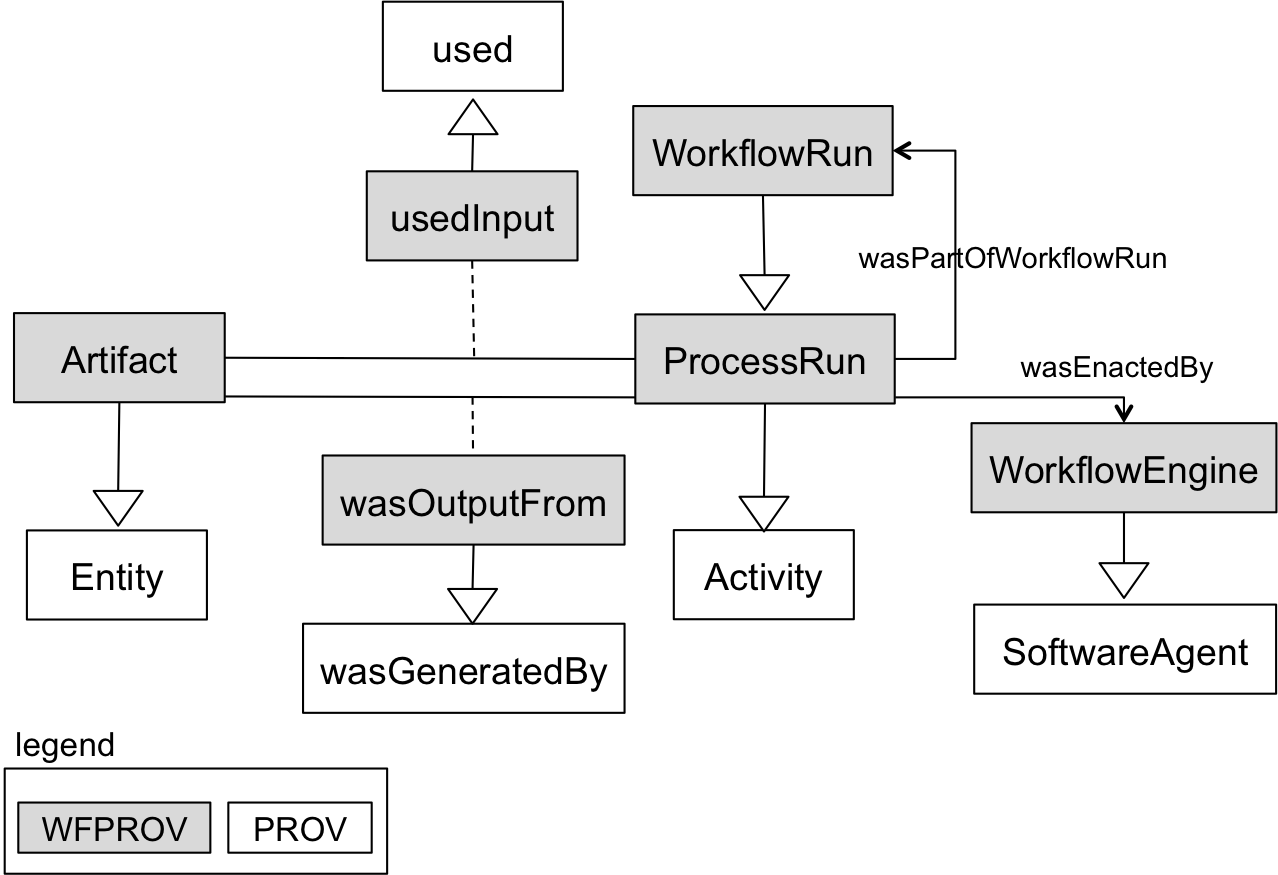
\includegraphics[width=0.6\textwidth]{Figures/wfprov.png}
  \caption{The \textit{wfprov} ontology.}
  \label{fig:wfprov}
\end{figure}

Figure \ref{fig:wfprov} illustrates the structure of the \textit{wfprov} ontology and its alignments with the W3C PROV-O ontology. A a workflow run~(\texttt{wfprov:WorkflowRun}) represents the enactment of a given workflow. It is composed of a set of process runs~(\texttt{wfprov:ProcessRun}), each representing the enactment of a process. A process run may use some artifacts~(\texttt{wfprov:Artifact}) as input and generate others as output. A process run is enacted by a workflow engine~(\texttt{wfprov:WorkflowEngine}), which can be seen as a PROV software agent.

By chaining the usage and generation of artifact together, the \textit{wfprov} ontology allows scientists to trace the lineage of workflow results. For example the user can identify the input artifacts that were used to feed the wokflow run (as a whole) to obtain a given output that was generated by the workflow run.

\paragraph{Tracking Research Object Evolution using the \textit{roevo} Vocabulary}
The \textit{roevo} ontology is another extension to the minimal core ontology for describing an important aspect of research objects, its life cycle.
%There are a number of existing work captures changes of information objects, like the changeset vocabulary, evolution of ontologies, like xxx, yyy, etc. 
To track the life cycle of a research object, we need to describe its changes at different levels of granularity, about the research object as a whole and about the individual resources. Also, we want to provide sufficient details to track the changes in order to roll back to a particular version or to quality control changes. Therefore, we need to describe when the change took place, who performed the change, and dependency relationships between the changes. %None of the existing vocabularies provide all the structure for us to build upon. 
Change is closely related to the provenance of a particular version of a research object or a resource. A study of the latest PROV-O ontology shows that it indeed provides all the foundational information elements for us to build the evolution ontology. 

\begin{figure}[ht]
  \centering
  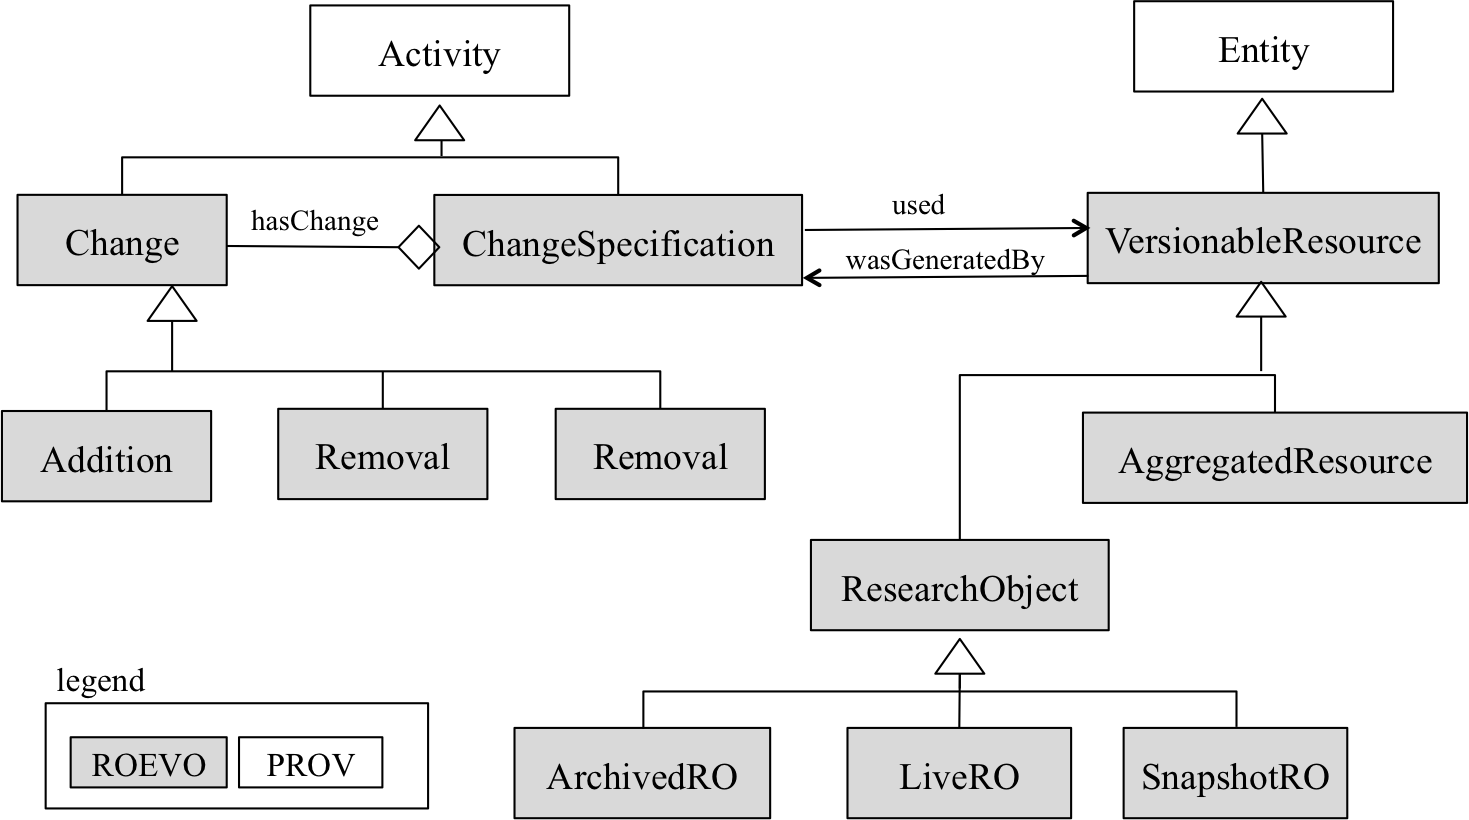
\includegraphics[width=0.6\textwidth]{Figures/roevo.png}
  \caption{The \textit{roevo} ontology extending PROV-O core terms.}
  \label{fig:ro_evo}
\end{figure}    

Figure~\ref{fig:ro_evo} illustrates the core concepts of this ontology and how it extends the PROV-O:
\begin{itemize}
\item To capture different status of a research object we create three sub-classes of \texttt{ro:ResearchObject}: the \texttt{roevo:LiveRO} is a research object to capture research findings during a live investigation and it can changed, and it can either archived or snapshotted. The \texttt{roevo:ArchivedRO} can be regarded as a production research object to be preserved and archived, such as one describing findings published in an article, and it can no longer be changed; the \texttt{roevo:SnapshotRO} represents a live Research Object at a particular time.
\item Both a snapshot of a live Research Object and an archived Research Object can be regarded as a versioned Research Object, i.e. a \texttt{roevo:VersionableResource}, Because it is a sub-class of \texttt{prov:Entity}, we can reuse PROV-O properties to describe the provenance or changes of this entity, such as pointing to the activity leading to any of its changes, the source research object that it was derived from, and the agent involved in its change.
\item A change is a \texttt{prov:Activity}, which means that it has a start time, an end time, an input entity and a resulting entity. Also a change leading to a new Research Object can constitute a series of changes. Therefore, we have a composite \texttt{roevo:ChangeSpecification} activity, which has a number of unit \texttt{roevo:Change}s. A unit change can be adding, removing or modifying a resource or a research object. But these different changes share the same pattern of taking an input entity and producing an output entity, which can all be nicely covered by properties from PROV-O.
\end{itemize}

As well as the above vocabularies, the Research Object model makes use of existing vocabularies, in particular, FOF\footnote{\url{http://xmlns.com/foaf/spec/}}, DCTerms\footnote{\url{http://dublincore.org/documents/dcmi-terms/}}, CITO\footnote{\url{http://vocab.ox.ac.uk/cito}}, and SCIOC\footnote{\url{http://sioc-project.org/ontology}} to provide Research Objects designers with the means to expresse aspects such as the people who were involved in the creation of a Research Object, its citation, as well as dependencies that the Research Object may have. For instance, we make use of the term \texttt{dc:requires} to specify that a the execution of a workflow requires other resources, e.g., plugins, credential, or specific execution environment.


\subsection{Research Object Manager}
\label{sec:romanager}

%% This section presents the RO manager architecture, and presents the functionalities it provides using  a UML sequence diagram, if that is plausible. 

The Research Object Manager (RO Manager) is a command line tool for creating, displaying and manipulating Research Objects. The RO Manager is complementary to RODL (see Section \ref{sec:rodl}), in that it is primarily designed to support a user working with ROs in the host computer's local file system, with the intention being that the RODL and RO Manager can exchange ROs between them, using of the shared RO model and vocabularies.  The RO Manager code base also includes the checklist evaluation functionality, described in D4.2 \cite{D4.2v2}, which can be invoked using a command line or REST web interface.

Experience has shown that a simple command-line tool can provide developers and users with early access to functionality, and provide an opportunity to gather additional user feedback and requirements.  RO Manager has also been used in conjunction with built-in operating system functionality for scripting prototype tool chains for more complex operations involving Research Objects.

The RO Manager allows users and developers to:

\begin{itemize}

\item Create local ROs;
\item Add resources to an RO;
\item Add annotations to an RO;
\item Read and write ROs to the RODL;
\item Perform checklist evaluation of an RO;
\item Obtain a raw dump of Research Object metadata.
\end{itemize}

To illustrate how the user can interact with the RO manager to manipulate Research Objects. Figure \ref{fig:romanagersequencediagram} shows interactions for three typical RO Manager operations, \texttt{ro create}, \texttt{ro add} and
\texttt{ro annotate}, which exemplify typical local RO management operations.

\begin{figure}
\begin{center}
\includegraphics[width=0.85\textwidth]{Figures/RO_Manager_seq.png}
\end{center}
\caption{RO Manager sequence diagram illustrating interactions with the user.}
\label{fig:romanagersequencediagram}
\end{figure}


The four interacting elements presented are the user-issued command (\texttt{/user}), the RO Manager program (\texttt{/RO\_Manager}), an internal RO metadata object (\texttt{/ro\_metadata}) that manages the RO aggregation and annotation metadata, and the local file system (\texttt{/file\_system}) where ROs are persistently stored and managed.

From this, it can be seen that:

\begin{itemize}

\item The \texttt{ro create} command initializes an RO structure by interacting directly with the file system.

\item The \texttt{ro add} command uses the RO URI to initialize an \texttt{ro$\_$metadata} object, and calls its \texttt{addAggregatedResources()} method to incorporate one or more files into the RO aggregation. The \texttt{ro$\_$metadata} object updates the RO metadata structures in the file system through a series or read and write operations.

\item The \texttt{ro annotate} command similarly uses the RO URI to initialize an \texttt{ro$\_$metadata} object, and reads the existing annotations from disk. New annotations may be supplied as an attribute/value or attribute/link pair in which a case a new annotation graph is created in the file system. Otherwise the new annotation may already exist as a graph. In either case, the local copy of the RO manifest is updated to record the new annotation. The annotation may be applied to multiple resources in the RO. Eventually, the updated manifest is written to the file system by the \texttt{ro$\_$metadata} object.
\end{itemize}

%\textbf{Source code organization:}
%\label{sourcecodeorganization:}

%The code base that implements the RO Manager command line tool also implements the checklist evaluation service, which is covered in D4.2 (@@ref)

%\begin{itemize}

%\item \texttt{Checklists/} - contains working data files used to develop and test checklist functionality
%\item \texttt{Minim/} - contains the OWL ontology descriptions of the Minim models used to describe a checklist to be evaluated by the evaluation service, and the results returned.  These are described further in D4.2 (@@ref)
%\begin{itemize}

%\item \texttt{doc/} - contains files for the RO Manager usage documentation
%\item \texttt{src/} - umbrella directory for the source code for RO Manager and the checklist evaluation service.  Also contains the script used to create and share an installable package for the RO Manager tool.
%\item \texttt{MiscLib/} - generic support functions
%\begin{itemize}

%\item test - unit tests
%\end{itemize}


%\item \texttt{iaeval/} - checklist evaluation functions, used by command line tool and evaluation web service.
%\begin{itemize}

%\item \texttt{test/} - unit tests
%\end{itemize}


%\item \texttt{rocommand/} - the main RO Manager command line tool, and also libraries used to access ROs by both the command line tool and the evaluation web service
%\begin{itemize}

%\item \texttt{test/} - unit tests, including a master test suite, TestAll.py, used for checking code prior to release.
%\end{itemize}


%\item \texttt{roweb/} - the checklist evaluation web service, and traffic light display: this is mainly a web front end to functionality implemented by modules in \texttt{rocommand} and \texttt{roweb}.
%\begin{itemize}

%\item \texttt{css/} - css and related files used by the web service
%\item \texttt{images/} - image files used by the web service
%\item \texttt{samples/} - miscellaneous sample and work-in-progress files, not part of the working software
%\item \texttt{test/} - unit tests
%\end{itemize}


%\item \texttt{samples/} - miscellaneous sample and work-in-progress files, not part of the working software
%\item \texttt{spike/} - code experiments, not part of working software
%\item \texttt{uritemplate/} - working copy of URI template expansion code from http://code.google.com/p/uri-templates/ (the package %has since been distributed via PyPI, so this local working copy should no longer be needed).
%\end{itemize}


%\end{itemize}

%\textbf{Key modules}
%\label{keymodules}

%Key modules that drive the execution of RO manager and the RO web services are:

%\begin{itemize}

%\item \texttt{src/ro} - a wrapper script to run the RO Manager command.
%\item \texttt{src/setup.py} - Python package creation and installation script.
%\item \texttt{src/rocommand/ro.py} - main command line interface for RO Manager, and command dispatcher.  Can be used directly, or invoked via \texttt{src/ro}.
%\item \texttt{src/rocommand/ro\_command.py} - functions to perform each of the RO Manager commands.
%\item \texttt{src/rocommand/ro\_manifest.py} - this is the key interface between RO Manager and the RO being constructed or examined.  Some access-only RO Manager commands can be performed against remote ROs (e.g. in RODL), and logic to detect and handle access to such remote ROs is included here.  This module provides the main internal API between application code and the RO, and as such provides a degree of isolation.
%\item \texttt{src/rocommand/ro\_manifest.py} - functions for accessing and manipulating an RO manifest in a local file store.
%\item \texttt{src/rocommand/ro\_annotation.py} - functions for creating, accessing and manipulating RO annotations in a local file store.
%\item \texttt{src/rocommand/ROSRS\_Session.py} - implements the RO API for accessing ROs in RODL (and possibly elsewhere).
%\item \texttt{src/roweb/rowebservices.py} - web interface for checklist evaluation and ``traffic-light'' display functions.
%\item \texttt{src/iaeval/ro\_eval\_minim.py} - checklist evaluation function (cf. \texttt{evaluate})
%\item \texttt{src/iaeval/ro\_minim.py} - Minim checklist definition access and parsing.
%\end{itemize}

%\textbf{Dependencies}
%\label{dependencies}

The RO manager is documented in a user guide that is available online\footnote{\url{http://wf4ever.github.io/ro-manager/doc/RO-manager.html}}.  An FAQ describing how to deal with various common operations using RO Manager is also accessible online \footnote{\url{http://www.wf4ever-project.org/wiki/display/docs/RO+Manager+FAQ}}.


The RO Manager is implemented in Python, and is available as an installable package through the Python Package Index (PyPI) \footnote{\url{https://pypi.python.org/pypi/ro-manager}}. The source code is maintained in the Wf4ever Github repository\footnote{\url{https://github.com/wf4ever/ro-manager}}.
The RO Manager is heavily dependent on \href{https://github.com/RDFLib}{RDFLib}\footnote{\href{https://github.com/RDFLib}{https://github.com/RDFLib}}, which provides RDF parsing, formatting and SPARQL Query capabilities. The RO Web service uses the \href{http://docs.pylonsproject.org/projects/pyramid/}{Pyramid}\footnote{\href{http://docs.pylonsproject.org/projects/pyramid/}{http://docs.pylonsproject.org/projects/pyramid/}} web framework, and \href{http://code.google.com/p/uri-templates/}{uritemplate}\footnote{\href{http://code.google.com/p/uri-templates/}{http://code.google.com/p/uri-templates/}} for \href{http://tools.ietf.org/html/rfc6570}{RFC 6570}\footnote{\href{http://tools.ietf.org/html/rfc6570}{http://tools.ietf.org/html/rfc6570}} template expansion.




\section{Research Object Digital Library}
\label{sec:rodl}

%This section presents the components that constitute the RODL, using a UML class diagram, and show how the user can utilize RODL using a UML sequence diagram.

The foundational service to preserve workflow-centric research objects is the Research Object Digital Library (RODL), which realizes the Storage and Lifecycle functionalities described in Section \ref{architecture}. It is a software system which collects, manages and preserves aggregations of scientific workflows and related objects and annotations, packed into research objects.

%\begin{figure*}[!hb]
%\centering
%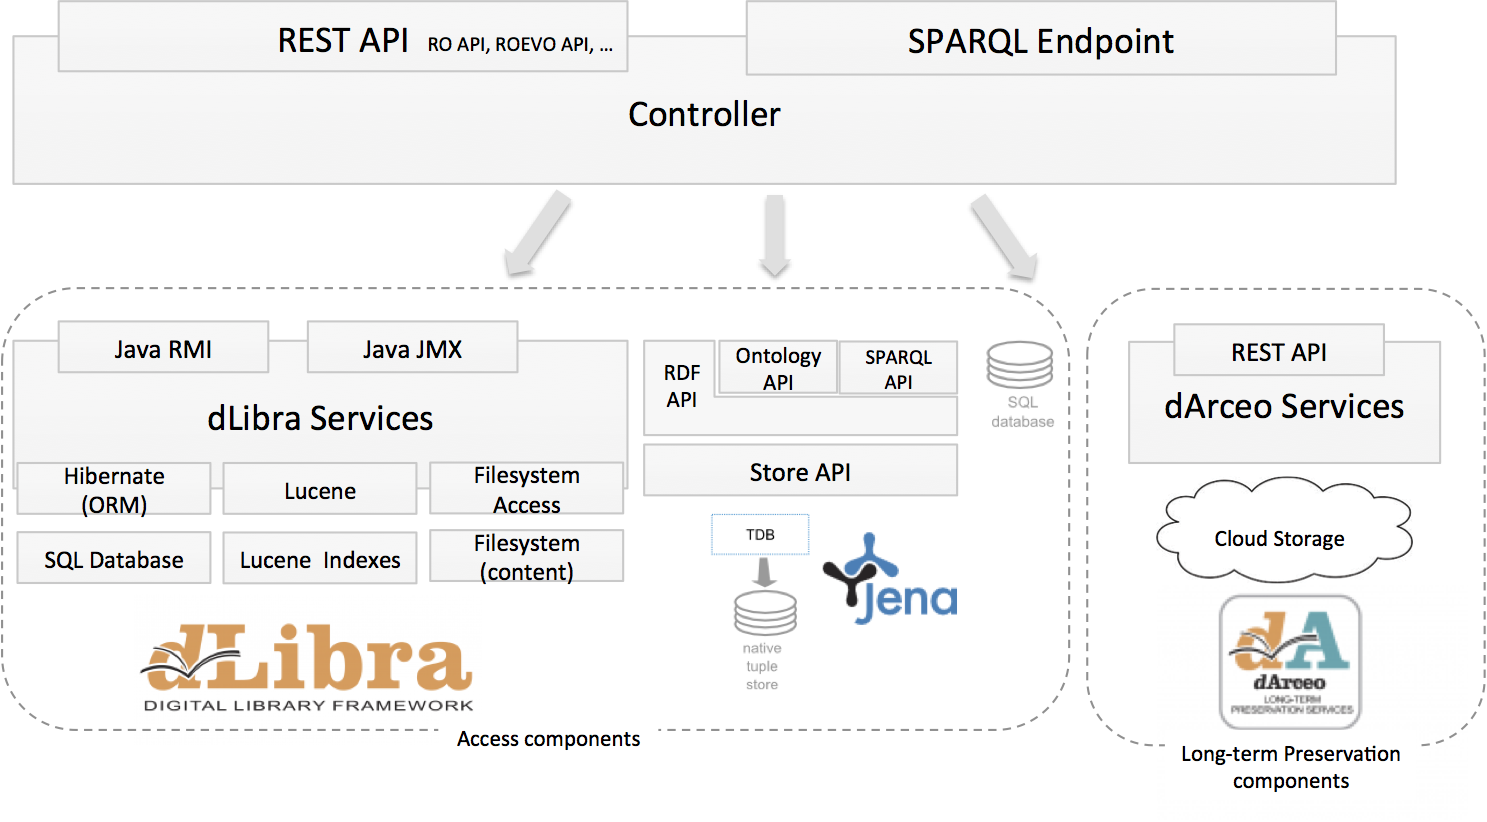
\includegraphics[width=\textwidth]{RODL-new.png}
%\caption{Research Objects Digital Library internal component diagram}
%\label{RODL}
%\end{figure*}


\subsection{The interfaces}

The main interface of RODL is a set of REST APIs, among which the two primary ones are the RO API \cite{RO-API} and the RO Evolution API \cite{RO-EVO-API}.

The RO API, also called the RO Storage and Retrieval API, defines the formats and links used to create and maintain research objects in the digital library. It is aligned with the RO model that is used to define research objects, and so it recognizes concepts such as aggregations, annotations and folders. The RO model ontology \cite{RO_model} is used to specify relations between different resources. Given that the semantic metadata are an important component of a research object, the RODL supports content negotiation for the metadata resources, including formats such as RDF/XML, Turtle and TriG.

The RO Evolution API defines the formats and links used to change the lifecycle stage of a research object, most importantly to create an immutable snapshot or archive from a mutable live research object, as well as to retrieve the evolution provenance of a research object. The API follows the RO evolution model \cite{w4fever_d321}, which is most visible in the evolution metadata that are generated for each state transition.

Additionally, RODL provides a SPARQL endpoint that allows performing SPARQL queries over HTTP to the metadata of all stored research objects. It also implements the Notification API \cite{Notification-API}, which defines links used to retrieve Atom feeds with notifications of events about any research object. For searching the contents of research objects a Solr REST API and the OpenSearch APIs are provided. Finally, RODL implements a custom User Management API \cite{UM-API} for registering users and generating OAuth 2 access tokens, providing the option of extending it with an access control layer in the future.

\begin{figure*}[!hb]
\centering
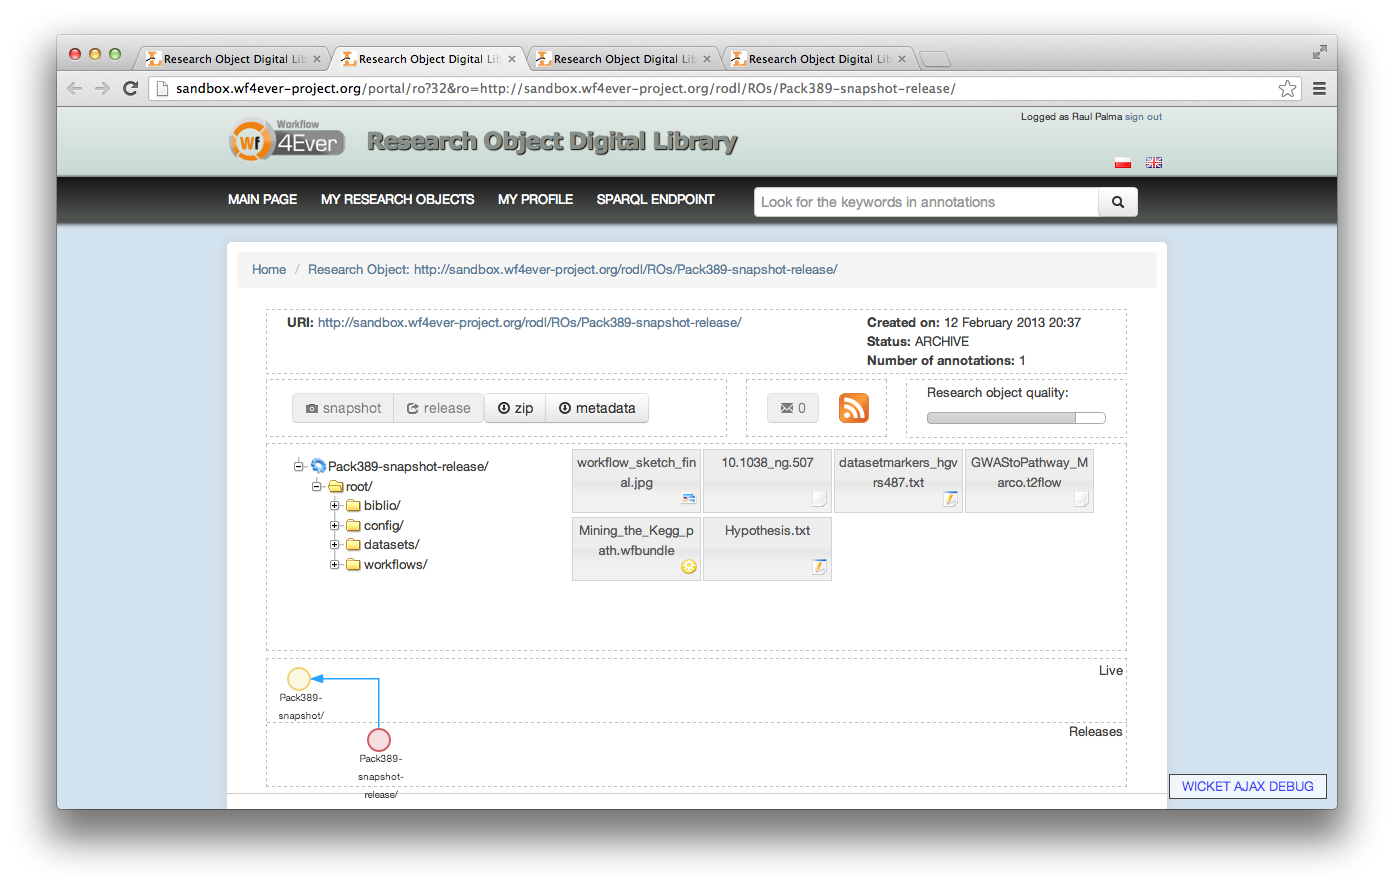
\includegraphics[width=0.98\textwidth]{RO-Portal-II.png}
\caption{The Research Object Portal}
\label{Portal}
\end{figure*}


\subsection{The implementation}

One of the main design challenges related to the implementation of RODL was the need to support both live, dynamically changing research objects as well as immutable snapshots that are intended for a longterm preservation. With this in mind, the RODL has a modular structure that comprises the access components, the longterm components and the controller that manages the flow of data (see figure \ref{RODL}). For immutable research objects, they are stored in the longterm preservation repository once they are created. The live research objects, on the other hand, are pushed asynchronously after every change or periodically, depending on the configuration.

The access components are the storage backend - dLibra \cite{dLibra} - and the semantic metadata triplestore. dLibra provides file storage and retrieval functionalities, including file versioning and consistency checking. It has a built-in text search engine and it manages users and controls their access rights. It allows organizing stored objects into hierarchical structures and associating metadata at the level of object aggregations. It is also possible to use a built-in module for storing research objects directly in the filesystem.

The semantic metadata are additionally parsed and stored in the triplestore backed by Jena TDB \cite{Jena}. Jena TDB is an actively developed RDF store implementation, which provides good support for transactions, querying, cacheing and using named graphs. The use of a triplestore helps in RODL internal data processing and offers a standard query mechanism for RODL clients. It also provides a flexible mechanism for storing metadata about any component of a research object that is identiable via a URI, which apart from workflows and other resources, may include parts of workflows or external resources (e.g. web services, data sources).

The longterm preservation component is built on dArceo \cite{dArceo} - a system for longterm preservation of digital objects developed by PSNC. dArceo stores the objects and monitors their quality, alerting the administrators if necessary. The standard monitoring activities include file format decay alerts and fixity checking but can be enhanced using a plugin mechanism. In case of RODL, dArceo monitors the quality of research objects by calling the Checklist Evaluation and Stability Services \cite{Checklist-API,Stability-API}. If a change in quality is detected, notifications are generated as Atom feeds in compliance with the Notification API mentioned above. This helps detect and prevent workflow decay which occurs when an external resource or service used by the workflow becomes unavailable or is otherwise behaving differently.

dArceo gives the possibility to define migration plans that allow to perform a batch update of resources from one format to another, when necessary. In case of workflows, this may be applied for instance when a flat Taverna t2flow format should be converted to a complex scufl2 format (which, notabene, uses the RO model similarly to research objects). Other case could be a batch update of workflows that depend on a malfunctioning external resource.

Objects in dArceo can be stored on a range of backends, including specialized preservation repositories such as the Platon service \cite{Platon}, storing data in geographically distributed copies and guaranteeing their consistency.

A running instance of the RODL is available for testing at \url{http://sandbox.wf4ever-project.org/rodl/}. At the moment of writing, it holds more than 1300 research objects.

\subsection{RODL clients}

The use of a REST API as the primary interface of RODL shows the need for clients that can facilitate the interaction with RODL for the users. To this moment, the following clients support some or all of the RO APIs implemented by RODL.

The reference client of RODL is \textbf{the RO Portal}, developed alongside RODL to test new features and expose all available functionalities. It is a web application running at \url{http://sandbox.wf4ever-project.org/portal}. Its main features are research object exploration and visualization; it also allows to create user accounts in RODL and generate access tokens for other clients. The RO Portal uses all APIs of RODL. Figure \ref{Portal} shows the main view of a research object in the RO Portal. The development version of \textbf{myExperiment} \cite{myExperiment} (\url{http://alpha.myExperiment.org}) uses RODL as a backend for storing packs. It uses the RO API. Finally, the \textbf{RO Manager} \cite{RO-Manager} is a command line tool that is primarily used to manage a research object stored on a local disk. It allows to push a research object to RODL via the RO API, as well as convert it into a snapshot in RODL.


\subsection{Research Object-Enabled myExperiment}
\label{sec:myexperiment}

%This section describes the efforts that went into incorporating research objects within myExperiment. In particular, how the notion of myExperiment pack was used as a starting point to incorporate new features/functionalaities. We will also discuss the diferent iterations that involved Wf4ever and Biovel users in those developments.

In this section, we describe how myExperiment \cite{DBLP:journals/fgcs/RoureGS09} was extended in order to cater for the sharing, publication and curation of Research Objects. myExperiment is a virtual research environment targeted towards collaborations for sharing and publishing workflows (and experiments). It provides the functionalities necessary for sharing workflows within and across multiple communities. In doing so, myExperiment adopts a social web approach, which is adapted to the need of scientists. The workflows that are shared using myExperiment do not need to be specified in a particular workflow management system. For example, we find on myExperiment workflows that have been specified using Galaxy \cite{galaxy}, Taverna \cite{taverna}, Kepler \cite{kepler} and Vistrails \cite{vistrails}.

\begin{figure}
\begin{center}
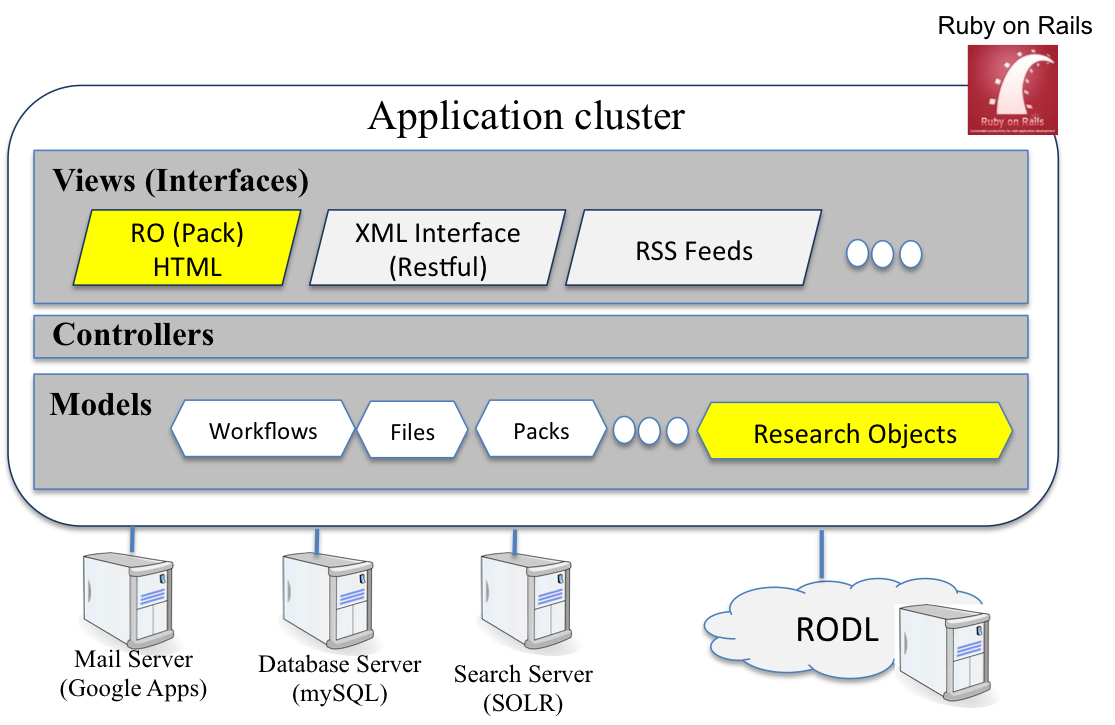
\includegraphics[width=0.7\textwidth]{Figures/myexperimentArchitecture.png}
\end{center}
\caption{RO-enabled myExperiment (except RODL, the modules in the above figure belong to the myExperiment infrastructure).}
\label{fig:myexperimentarchitecture}
\end{figure}


While initially targeted towards workflows, the creators of myExperiment were aware that scientists want to share more than just workflows and experiments. Because of this, myExperiemnt was extended to support the sharing of artifacts known as Packs. A pack can be seen as a basic aggregation of resources, which can be workflows, but also files, presentations, papers, or links to external resources. 
The notion of packs has been widely adopted by scientists. At the time of writing, myExperiment had $337$ packs. Just like a workflow, using myExperiment a pack can be annotated and shared. 
 
\begin{figure}
\begin{center}
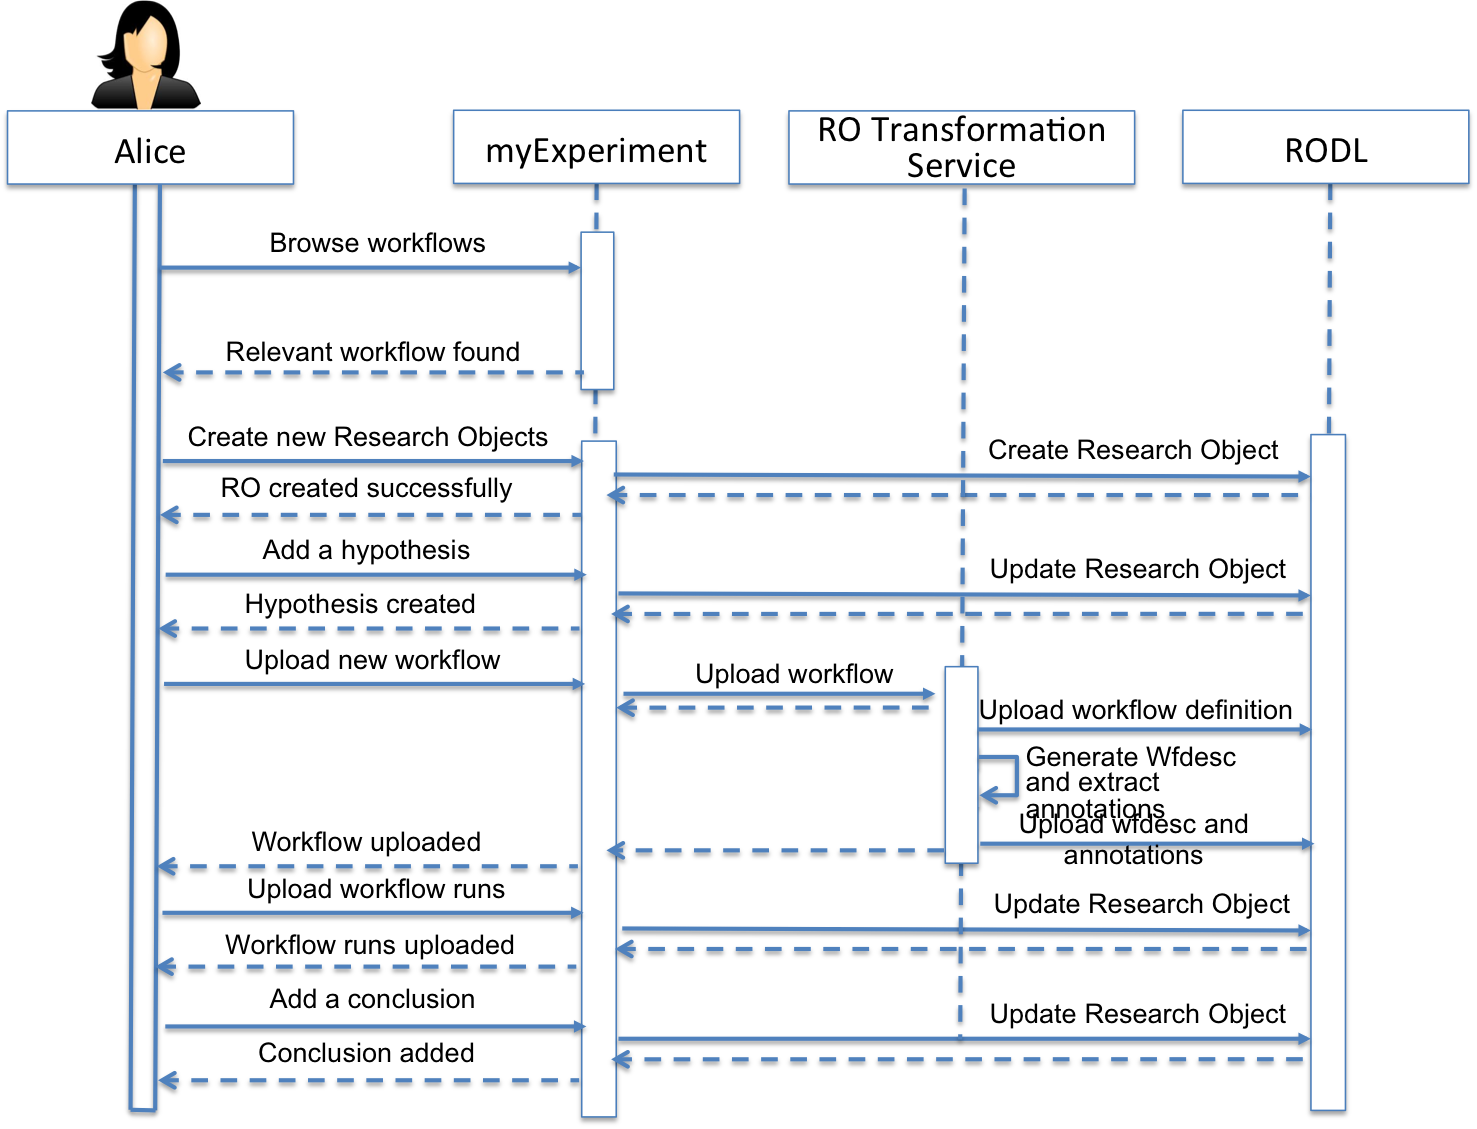
\includegraphics[width=0.7\textwidth]{Figures/myexperimentInteractions.png}
\end{center}
\caption{A Sequence diagram illustrating how myExperiment can be used to create Research Objects.}
\label{fig:myexperimentinteractions}
\end{figure} 
 
In order to support complex forms of sharing, reuse and preservation, we have worked during the last year on incorporating the notion of Research Objects (which can be seen as advanced packs) into the development version of myExperiment \footnote{http://alpha.myexperiment.org/packs/}. In addition to the basic aggregation supported by packs, alpha myExperiment\footnote{It is worth noting that once the development in the myExperiment alpha is judged mature, the new functionalities will be staged to the production version of myExperiment.} provides the mechanisms for specifying metadata that describes the relationships between the resources within the aggregation. Moreover, the structure and the types of the resources that compose a pack are now inline with those that have been identified thanks to the Research Object model. For example, a user is able to specify that a given file within a pack specifies the hypothesis, that another file specifies the workflow run obtained by enacting a given workflow, or that a given file states the conclusions drawn by the scientists after analyzing the workflow run.


Figure \ref{fig:myexperimentarchitecture} illustrates a high-level architecture of alpha myExperiment, the development version of myExperiment into which the Research Objects capabilities were incorporated. As illustrated in the figure, at the level of the Rails\footnote{\url{http://rubyonrails.org}} model, data structures that represent the Research Object and associated resources have been incorporated. To manipulate such data structures, the controller layer has been extended, and to provide non-information technology users with the ability to create and manage Research Objects, the view layer has been extended with the necessary HTML Web pages.



To illustrate how myExperiment can be used for managing Research Objects, Figure \ref{fig:myexperimentinteractions} depicts a sequence UML diagram illustrating a typical sequence of interactions that the user undergoes to create and share a Research Object. Alice (the user) first browses myExperiment to identify a workflow that is of interest to her investigation. Once she identified a relevant workflow, she downloads the workflow, modifies and re-purposes it for her investigation. Once she is happy with the \emph{new} workflow, Alice decides to create a Research Object. In doing so, she specifies the hypothesis within a file, which is stored within RODL. RODL acts as a back-end for myExperiment to store the information about Research Objects. Alice then uploads her workflow to myExperiment. As a result, myExperiment sends a request to the \texttt{RO transformation service}, which uploads the workflow definition to RODL, transforms the workflow definition into wfdesc, and extracts the annotations that are bundled within the workflow definition. These elements, i.e., wfdesc specification and annotations, are then uploaded to the Research Object in RODL. Alice also uploads the workflow runs obtained as a result of enacting her workflow, and specifies the conclusion she comes to at the end of her investigation. 

Using myExperiment, Alice now has a Research Object, compliant with the models from Section \ref{sec:romodel}, viewable and manipulable as a pack through myExperiment, and enriched with a hypothesis and conclusions that can assist other users in understanding and possibly reusing and re-purposing her research results.


\section{Workflow Abstraction using Motifs}
This section presents the motif ontology, again using a UML class diagram, and provides an example of a workflow that was annotated using the motifs.

\section{Indexing Workflows}
\label{sec:indexation}

This section shows how workflows have been indexed using a generalized trie structure\footnote{Trie comes from the word re{\bf Trie}val indicating the process of information accessing but it is also called suffix tree.} and a serialization process. 
%Workflows are a common way of providing and preserving scientific methods by explicitly encoding their processes. They are defined as directed acyclic graphs (DAG) and in Wf4Ever have been described by using both wfdesc and wfprov vocabularies. Therefore, 
A workflow $wf$ can be defined as a set of $Processes_{wf}$ and $Params_{wf} \quad | \quad wf = Processes_{wf} \cup Params_{wf}$ where the $Processes_{wf}$ are the definition of specific tasks to be executed, and $Params_{wf}$ defines the inputs and outputs of those tasks. On the other hand, a trie structure is an ordered tree data structure that allows to store dynamically a vector or an associative array where the keys are the values being stored itself. The main characteristic of this structure is absence of tree nodes being used for storing the key associated with that node but the position of the node within the tree defines the key. Another characteristic of this structure is that all the descendants of a node have a common prefix and therefore allows indexing simultaneously complete or partial paths to a specific node. \\

For our purposes of indexing a workflow, or generally speaking any DAG, by using a trie structure as a sequence of items which represents the DAG partially or completely for later accessing, a preprocessing of the set of workflows is needed as a first step. For accomplishing with this preprocessing goal of adapting a DAG to the trie indexing structure we have used one of the possible topological orders of a DAG. It is known that any DAG has at least one topological ordering which assures that if a vertex $u$ is linked through an edge to vertex $v$, then after sorting it the vertex $u$ will come before $v$ in ordering. This topological ordering does not have to be unique and therefore a DAG could be defined by multiple topological sorts. Similarly to~\cite{Matono03anindexing}, in order to avoid the possibility of having similar workflows defined in  different ways within the same indexing structure, we have chosen the lexicographical order of processes as common criteria to be applied. Therefore, the chosen overall used criteria for ordering the DAG sequentially has been both the topological and lexicographical orders. \\

The figure~\ref{fig:sorting-workflow} shows how the "Extract proteins using a gi - output as fasta file"\footnote{http://www.myexperiment.org/workflows/1182.html} example which was obtained from ProvBench data set~\cite{khalid_13}, is sorted by applying our criteria. One of the main advantages of this approach is that after transforming the DAG workflow into a sequential linked set of resources it can be indexed almost instantaneously and the time for searching and exact matching is linear with the size of the tree which is also directly related to the vocabulary size of the domain.

\begin{figure*}[ht!]
\centering
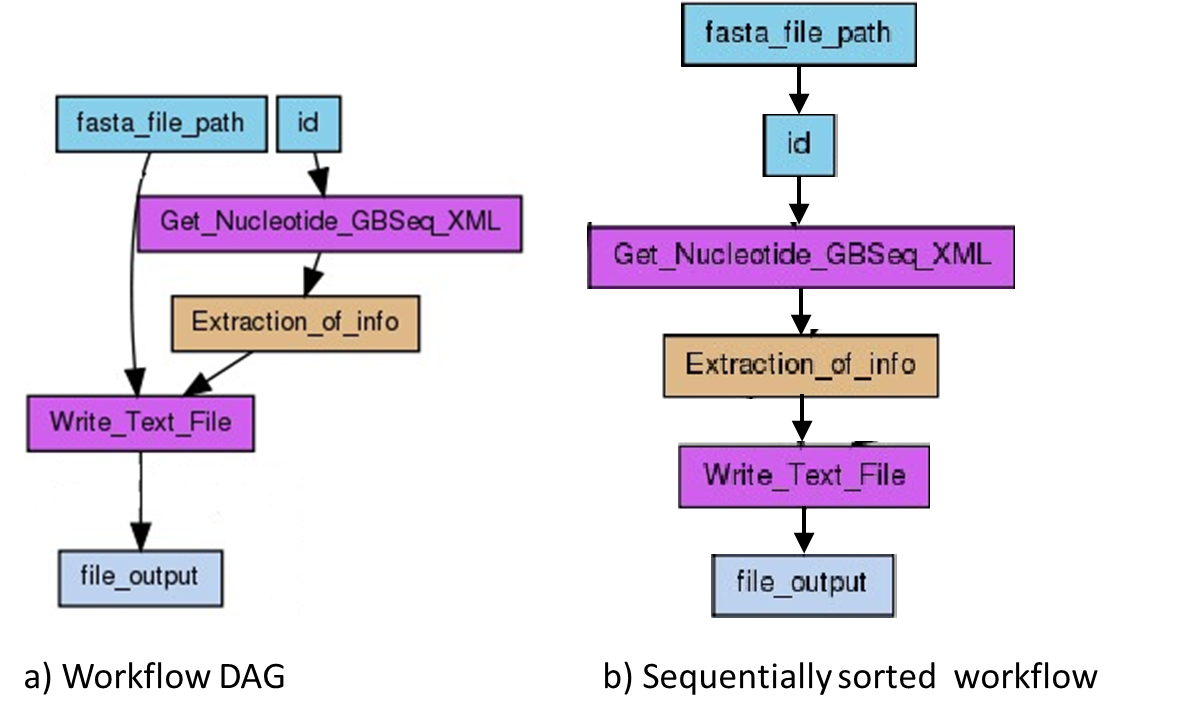
\includegraphics[scale=0.70]{Figures/sorting-workflow.png}
\caption{\textcolor{black}{Sorting the "Extract proteins using a gi - output as fasta file" example obtained from ProvBench}}
\label{fig:sorting-workflow}
\end{figure*}

\subsection{Applications and Implementation}
In order to provide scientists with searching and design capabilities we have implemented two different web services which makes use of the above introduced indexing structure for accessing to workflows and recommend next steps given the previous ones. It is worth highlighting that the implemented indexing structure could be also used for other purposes as the discovery of frequent patterns by using the collected statistical information and mining the semantic trie structure which would take full advantage of the intrinsic sequential ordering of the trie structure. 

The implementation of both services (searching and next step recommendation) has been done applying the guidelines of the Wf4Ever project. Both services are REST and can be called by an HTTP GET method which upon on ACCEPT headers may return XML or JSON formats. Also for implementation purposes we have encapsulated the trie indexing structured in order to provided the above presented services.
 
\subsubsection{Searching}

This service\footnote{\url{http://sandbox.wf4ever-project.org/wfabstraction/rest/search}} searches for those workflows which contain a specific sequence of processes providing on real time a list including all of them. The service accepts an array of processes' names as input parameter process[] (e.g. process?=p1\&p2\&p3). Therefore the general call would be of the form\footnote{\url{http://sandbox.wf4ever-project.org/wfabstraction/rest/search{?process[]}}}:\\

The output is an XML or JSON structure with the following attributes: 
\begin{itemize}
\item \textbf{Process\_id}: is the name of the process or processes used in the query.
\item \textbf{freq}: is the number of times that the sequence of processes appears in other workflows.
\item \textbf{URIs}: are the URIs of the workflows where the sequence appears. 
\end{itemize}

\subsubsection{Next step recommendation}
The proposed trie structure captures the provenance of workflows execution associated to scientific experiments allowing
their indexation based on the temporal information that they contain. The trie structure is also updated to gather
the needed statistics for mining the execution of workflows and provide the recommended next process based on how frequent 
a pattern of use occurs. So far we collected the number of times a process occurs in the dataset and also the probability associated 
to that pattern given the set of patterns of the same size. The fact that the exact matching searching is linear with the size of the tree (which is dependent of the use vocabulary, in our case the domain has been restricted to the set of processes included in ProvBench~\cite{khalid_13}) makes it very suitable for 
this type of applications. The implemented service\footnote{\url{http://sandbox.wf4ever-project.org/wfabstraction/rest/recommend}} accepts an array of processes' names as input parameter process[] (e.g. process?=p1\&p2\&p3) and its general call would be of the form\footnote{\url{http://sandbox.wf4ever-project.org/wfabstraction/rest/recommend{?process[]}}}: \\

The output is an XML or JSON structure with different attributes:
\begin{itemize}
\item \textbf{Id}: is the name of the recommended process for that input query.
\item \textbf{freq}:  is the number of times that it appears in different workflows.
\item \textbf{prob}:  is the probability of the given recommendation taking into account the whole set of possible next steps.
\end{itemize}

\section{Summary}
\label{sec:conclusions}

We have presented in this deliverable the final version Research Object model defined within Wf4Ever, as a family of ontologies. We also presented the tools that were built on the model in order to facilitate the creation, curation and sharing of Research Objects, namely, the Research Object Manager (RO Manager), a command line tool for creating, displaying and manipulating Research Objects, RODL, which acts as a back-end, with two storage alternatives: a digital repository to keep the content, as a triple store to manage the metadata content, and the myExperiment virtual research environment, which was extended to allow end-users to create, upload, share and curate Research Objects. We also presented two models that cater for advanced functionalities, namely abstracting and indexing workflows.

Our ongoing and future work aims to advertise and disseminate the Research Object model and the tools developed around it. In this respect, it is worth mentioning that we have launched a website dedicated to Research Objects\footnote{\url{http://www.researchobject.org/}}, with examples that assist prospective adopters in understanding the model usage and benefits.


\appendix
\clearpage
\addcontentsline{toc}{section}{Bibliography}
\bibliographystyle{alpha}
\bibliography{refs.bib}
%------------------------------------------------------------------------------------------------------
%Keep following label in order for Latex to get the total number of pages right
%---
\label{lastpage}
%---
\end{document}
